\subsect{Sprint 4}{sprint4}

\underline{Fecha de inicio}: 11/09/2022

\underline{Fecha de fin}: 11/10/2022

\underline{Objetivos}:
\begin{itemize}
	\item Añadir soporte para el envío de archivos.
	\item Utilizar Docker para la aplicación.
\end{itemize}

\underline{Descripción}:
En este sprint se añadirá soporte para el envío de archivos multimedia en los mensajes.\ Se limitará el tamaño de
los archivos a 30 MB, para evitar que se envíen archivos demasiado grandes.\ Además, se utilizará Docker para
la aplicación, de forma que se pueda desplegar fácilmente en cualquier servidor.\ Esto también facilita la integración
entre todos los servicios utilizados en la aplicación, ya que se pueden desplegar todos a la vez con un solo
comando.\ Se ha realizado la migración de la aplicación a un servidor personal, debido a que Heroku ha eliminado
su plan gratuito, como se ha comentado en el sprint anterior.\ Para más información, consultar la
sección~\ref{subsec:deployment_problems}.

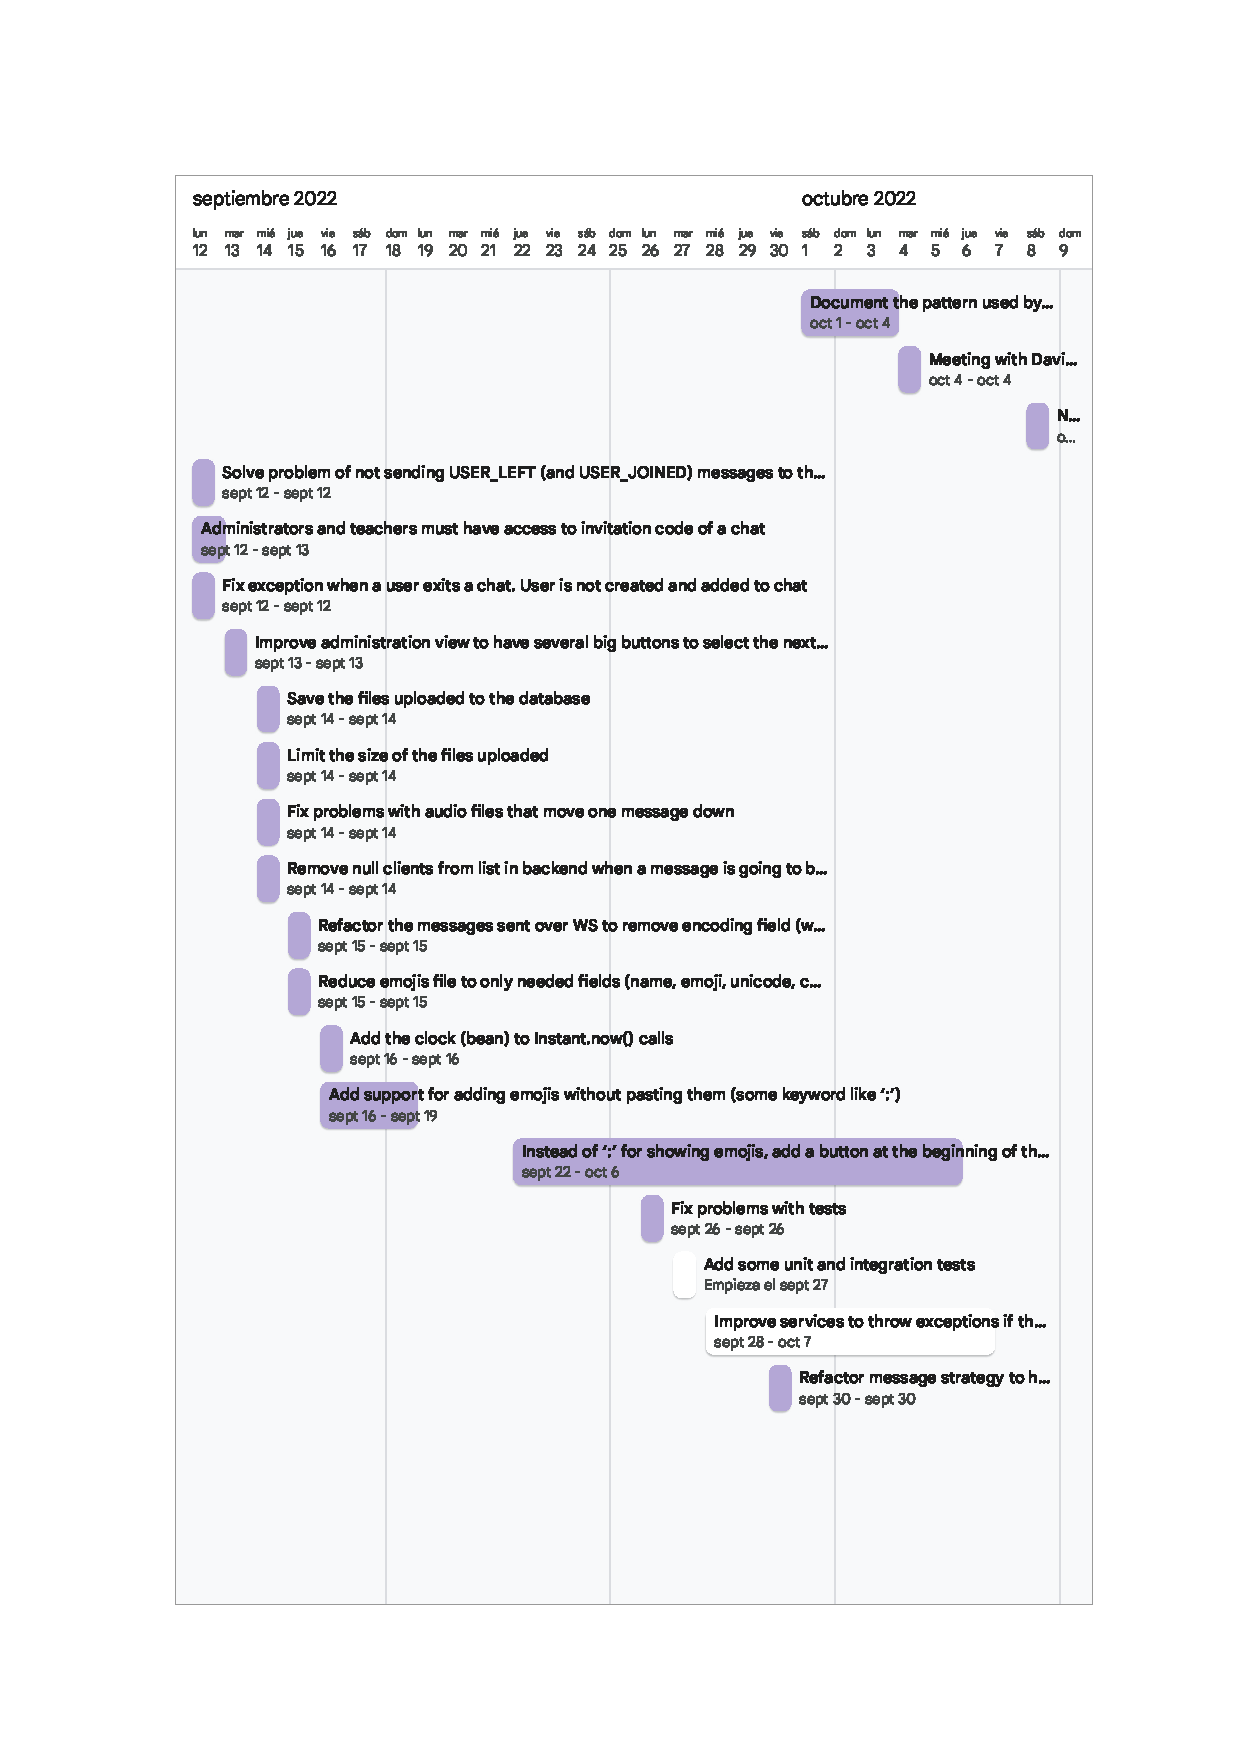
\includepdf[pages=-]{backlog/sprints/Sprint4.pdf}
